%% bm.pdf preamble - material merged from previous preamble and current pandoc preamable output
% NOTE: float placement required changes to the source files referenced by bm.tex
% May 28, 2020
%
% Use lualatex to compile - test with MiKTeX 2.9

% uncomment to list all files in log
%\listfiles

\documentclass[12pt]{report}


\usepackage{fontspec}

%\setmainfont[Scale=MatchLowercase]{Lucida Bright}
%\setmonofont{FreeMono}
%\setmonofont{Source Code Pro}
\setmonofont[Scale=MatchLowercase]{Ubuntu Mono}

% short snippets of asian languages
\newfontfamily\myAsian{Noto Serif TC Medium}

\usepackage[headings]{fullpage}

% national use characters 
%\usepackage{inputenc}

% ams mathematical symbols
\usepackage{amsmath,amssymb}

% added to support pandoc highlighting
\usepackage{microtype}

\usepackage{makeidx}

% add index and bibliographies to table of contents
\usepackage[nottoc]{tocbibind}

% postscript courier and times in place of cm fonts
%\usepackage{courier}
%\usepackage{times}

% extended coloring
\usepackage{color}
\usepackage[table,dvipsnames]{xcolor}
\usepackage{colortbl}

% advanced date formating
\usepackage{datetime}

%support pandoc code highlighting
\usepackage{fancyvrb}

% \DefineShortVerb[commandchars=\\\{\}]{\|}
% \DefineVerbatimEnvironment{Highlighting}{Verbatim}{commandchars=\\\{\}}
% % Add ',fontsize=\small' for more characters per line

% tango style colors
% \usepackage{framed}
% \definecolor{shadecolor}{RGB}{255,255,255}
% \newenvironment{Shaded}{\begin{snugshade}}{\end{snugshade}}
% \newcommand{\KeywordTok}[1]{\textcolor[rgb]{0.13,0.29,0.53}{\textbf{{#1}}}}
% \newcommand{\DataTypeTok}[1]{\textcolor[rgb]{0.13,0.29,0.53}{{#1}}}
% \newcommand{\DecValTok}[1]{\textcolor[rgb]{0.00,0.00,0.81}{{#1}}}
% \newcommand{\BaseNTok}[1]{\textcolor[rgb]{0.00,0.00,0.81}{{#1}}}
% \newcommand{\FloatTok}[1]{\textcolor[rgb]{0.00,0.00,0.81}{{#1}}}
% \newcommand{\CharTok}[1]{\textcolor[rgb]{0.31,0.60,0.02}{{#1}}}
% \newcommand{\StringTok}[1]{\textcolor[rgb]{0.31,0.60,0.02}{{#1}}}
% \newcommand{\CommentTok}[1]{\textcolor[rgb]{0.56,0.35,0.01}{\textit{{#1}}}}
% \newcommand{\OtherTok}[1]{\textcolor[rgb]{0.56,0.35,0.01}{{#1}}}
% \newcommand{\AlertTok}[1]{\textcolor[rgb]{0.94,0.16,0.16}{{#1}}}
% \newcommand{\FunctionTok}[1]{\textcolor[rgb]{0.00,0.00,0.00}{{#1}}}
% \newcommand{\RegionMarkerTok}[1]{{#1}}
% \newcommand{\ErrorTok}[1]{\textbf{{#1}}}
% \newcommand{\NormalTok}[1]{{#1}}

% %espresso style colors
% \usepackage{framed}
% \definecolor{shadecolor}{RGB}{42,33,28}
% \newenvironment{Shaded}{\begin{snugshade}}{\end{snugshade}}
% \newcommand{\KeywordTok}[1]{\textcolor[rgb]{0.26,0.66,0.93}{\textbf{{#1}}}}
% \newcommand{\DataTypeTok}[1]{\textcolor[rgb]{0.74,0.68,0.62}{\underline{{#1}}}}
% \newcommand{\DecValTok}[1]{\textcolor[rgb]{0.27,0.67,0.26}{{#1}}}
% \newcommand{\BaseNTok}[1]{\textcolor[rgb]{0.27,0.67,0.26}{{#1}}}
% \newcommand{\FloatTok}[1]{\textcolor[rgb]{0.27,0.67,0.26}{{#1}}}
% \newcommand{\CharTok}[1]{\textcolor[rgb]{0.02,0.61,0.04}{{#1}}}
% \newcommand{\StringTok}[1]{\textcolor[rgb]{0.02,0.61,0.04}{{#1}}}
% \newcommand{\CommentTok}[1]{\textcolor[rgb]{0.00,0.40,1.00}{\textit{{#1}}}}
% \newcommand{\OtherTok}[1]{\textcolor[rgb]{0.74,0.68,0.62}{{#1}}}
% \newcommand{\AlertTok}[1]{\textcolor[rgb]{1.00,1.00,0.00}{{#1}}}
% \newcommand{\FunctionTok}[1]{\textcolor[rgb]{1.00,0.58,0.35}{\textbf{{#1}}}}
% \newcommand{\RegionMarkerTok}[1]{\textcolor[rgb]{0.74,0.68,0.62}{{#1}}}
% \newcommand{\ErrorTok}[1]{\textcolor[rgb]{0.74,0.68,0.62}{\textbf{{#1}}}}
% \newcommand{\NormalTok}[1]{\textcolor[rgb]{0.74,0.68,0.62}{{#1}}}

% %kete style colors
% \newenvironment{Shaded}{}{}
% \newcommand{\KeywordTok}[1]{\textbf{{#1}}}
% \newcommand{\DataTypeTok}[1]{\textcolor[rgb]{0.50,0.00,0.00}{{#1}}}
% \newcommand{\DecValTok}[1]{\textcolor[rgb]{0.00,0.00,1.00}{{#1}}}
% \newcommand{\BaseNTok}[1]{\textcolor[rgb]{0.00,0.00,1.00}{{#1}}}
% \newcommand{\FloatTok}[1]{\textcolor[rgb]{0.50,0.00,0.50}{{#1}}}
% \newcommand{\CharTok}[1]{\textcolor[rgb]{1.00,0.00,1.00}{{#1}}}
% \newcommand{\StringTok}[1]{\textcolor[rgb]{0.87,0.00,0.00}{{#1}}}
% \newcommand{\CommentTok}[1]{\textcolor[rgb]{0.50,0.50,0.50}{\textit{{#1}}}}
% \newcommand{\OtherTok}[1]{{#1}}
% \newcommand{\AlertTok}[1]{\textcolor[rgb]{0.00,1.00,0.00}{\textbf{{#1}}}}
% \newcommand{\FunctionTok}[1]{\textcolor[rgb]{0.00,0.00,0.50}{{#1}}}
% \newcommand{\RegionMarkerTok}[1]{{#1}}
% \newcommand{\ErrorTok}[1]{\textcolor[rgb]{1.00,0.00,0.00}{\textbf{{#1}}}}
% \newcommand{\NormalTok}[1]{{#1}}
% %end pandoc code hacks

% jodliterate colors
\usepackage{color}
\definecolor{shadecolor}{RGB}{248,248,248}
% j control structures 
\definecolor{keywcolor}{rgb}{0.13,0.29,0.53}
% j explicit arguments x y m n u v
\definecolor{datacolor}{rgb}{0.13,0.29,0.53}
% j numbers - all types see j.xml
\definecolor{decvcolor}{rgb}{0.00,0.00,0.81}
\definecolor{basencolor}{rgb}{0.00,0.00,0.81}
\definecolor{floatcolor}{rgb}{0.00,0.00,0.81}
% j local assignments
\definecolor{charcolor}{rgb}{0.31,0.60,0.02}
\definecolor{stringcolor}{rgb}{0.31,0.60,0.02}
\definecolor{commentcolor}{rgb}{0.56,0.35,0.01}
% primitive adverbs and conjunctions
%\definecolor{othercolor}{rgb}{0.56,0.35,0.01}   
\definecolor{othercolor}{RGB}{0,0,255}
% global assignments
\definecolor{alertcolor}{rgb}{0.94,0.16,0.16}
% primitive J verbs and noun names
\definecolor{funccolor}{rgb}{0.00,0.00,0.00}

% custom colors
\definecolor{CodeBackGround}{cmyk}{0.0,0.0,0,0.05}    % light gray
\definecolor{CodeComment}{rgb}{0,0.50,0.00}           % dark green {0,0.45,0.08}
\definecolor{TableStripes}{gray}{0.9}                 % odd/even background in tables

% Colors for the hyperref package
\definecolor{urlcolor}{rgb}{0,.145,.698}
\definecolor{linkcolor}{rgb}{.71,0.21,0.01}
\definecolor{citecolor}{rgb}{.12,.54,.11}

% % Exact colors from NB
\definecolor{incolor}{HTML}{303F9F}
\definecolor{outcolor}{HTML}{D84315}
\definecolor{cellborder}{HTML}{CFCFCF}
\definecolor{cellbackground}{HTML}{F7F7F7}

% % ANSI colors
\definecolor{ansi-black}{HTML}{3E424D}
\definecolor{ansi-black-intense}{HTML}{282C36}
\definecolor{ansi-red}{HTML}{E75C58}
\definecolor{ansi-red-intense}{HTML}{B22B31}
\definecolor{ansi-green}{HTML}{00A250}
\definecolor{ansi-green-intense}{HTML}{007427}
\definecolor{ansi-yellow}{HTML}{DDB62B}
\definecolor{ansi-yellow-intense}{HTML}{B27D12}
\definecolor{ansi-blue}{HTML}{208FFB}
\definecolor{ansi-blue-intense}{HTML}{0065CA}
\definecolor{ansi-magenta}{HTML}{D160C4}
\definecolor{ansi-magenta-intense}{HTML}{A03196}
\definecolor{ansi-cyan}{HTML}{60C6C8}
\definecolor{ansi-cyan-intense}{HTML}{258F8F}
\definecolor{ansi-white}{HTML}{C5C1B4}
\definecolor{ansi-white-intense}{HTML}{A1A6B2}
\definecolor{ansi-default-inverse-fg}{HTML}{FFFFFF}
\definecolor{ansi-default-inverse-bg}{HTML}{000000}
    

% \usepackage{framed}
% \newenvironment{Shaded}{}{}
% \newcommand{\KeywordTok}[1]{\textcolor{keywcolor}{\textbf{{#1}}}}
% \newcommand{\DataTypeTok}[1]{\textcolor{datacolor}{{#1}}}
% %\newcommand{\DecValTok}[1]{\textcolor{decvcolor}{{#1}}}
% \newcommand{\DecValTok}[1]{{#1}} 
% \newcommand{\BaseNTok}[1]{\textcolor{basencolor}{{#1}}}
% \newcommand{\FloatTok}[1]{\textcolor{floatcolor}{{#1}}}
% \newcommand{\CharTok}[1]{\textcolor{charcolor}{\textbf{{#1}}}}
% \newcommand{\StringTok}[1]{\textcolor{stringcolor}{{#1}}}
% \newcommand{\CommentTok}[1]{\textcolor{commentcolor}{\textit{{#1}}}}
% \newcommand{\OtherTok}[1]{\textcolor{othercolor}{{#1}}} 
% \newcommand{\AlertTok}[1]{\textcolor{alertcolor}{\textbf{{#1}}}}
% %\newcommand{\FunctionTok}[1]{\textcolor{funccolor}{{#1}}}
% \newcommand{\FunctionTok}[1]{{#1}}
% \newcommand{\RegionMarkerTok}[1]{{#1}}
% \newcommand{\ErrorTok}[1]{\textbf{{#1}}}
% \newcommand{\NormalTok}[1]{{#1}}

% The default LaTeX title has an obnoxious amount of whitespace. By default,
% titling removes some of it. It also provides customization options.
\usepackage{titling}

% headers and footers
\usepackage{fancyhdr}
%\pagestyle{fancy}
\pagestyle{plain}

\fancyhead{}
\fancyfoot{}

%\fancyhead[LE,RO]{\slshape \rightmark}
%\fancyhead[LO,RE]{\slshape \leftmark}
\fancyfoot[C]{\thepage}
%\headrulewidth 0.4pt
%\footrulewidth 0 pt

%\addtolength{\headheight}{\baselineskip}

%\lfoot{\emph{Analyze the Data not the Drivel}}
%\rfoot{\emph{\today}}

% subfigure handles figures that contain subfigures
%\usepackage{color,graphicx,subfigure,sidecap}
\usepackage{graphicx,sidecap}
\usepackage{subfigure}
\graphicspath{{./inclusions/}}

% floatflt provides for text wrapping around small figures and tables
\usepackage{floatflt}

% tweak caption formats 
\usepackage{caption} 
\usepackage{sidecap}
%\usepackage{subcaption} % not compatible with subfigure

\usepackage{rotating} % flip tables sideways

% complex footnotes
%\usepackage{bigfoot}

% weird logos \XeLaTeX
\usepackage{metalogo}

\newcommand{\HRule}{\rule{\linewidth}{0.5mm}}

\usepackage[breakable]{tcolorbox}

\usepackage{parskip} % Stop auto-indenting (to mimic markdown behaviour)
    
% Basic figure setup, for now with no caption control since it's done
% automatically by Pandoc (which extracts ![](path) syntax from Markdown).
\usepackage{graphicx}

%\DeclareCaptionFormat{nocaption}{}
%\captionsetup{format=nocaption,aboveskip=0pt,belowskip=0pt}

\usepackage[Export]{adjustbox} % Used to constrain images to a maximum size
\adjustboxset{max size={0.9\linewidth}{0.9\paperheight}}
\usepackage{float}

%\floatplacement{figure}{H} % forces figures to be placed at the correct location

\usepackage{xcolor} % Allow colors to be defined
\usepackage{enumerate} % Needed for markdown enumerations to work
\usepackage{geometry} % Used to adjust the document margins

%\usepackage{amsmath} % Equations
%\usepackage{amssymb} % Equations

\usepackage{textcomp} % defines textquotesingle

% Hack from http://tex.stackexchange.com/a/47451/13684:
\AtBeginDocument{%
	\def\PYZsq{\textquotesingle}% Upright quotes in Pygmentized code
}

\usepackage{upquote} % Upright quotes for verbatim code
\usepackage{eurosym} % defines \euro
\usepackage[mathletters]{ucs} % Extended unicode (utf-8) support

%\usepackage{fancyvrb} % verbatim replacement that allows latex

\usepackage{grffile} % extends the file name processing of package graphics 
					 % to support a larger range
					 
\makeatletter % fix for grffile with XeLaTeX
\def\Gread@@xetex#1{%
  \IfFileExists{"\Gin@base".bb}%
  {\Gread@eps{\Gin@base.bb}}%
  {\Gread@@xetex@aux#1}%
}
\makeatother

% The hyperref package gives us a pdf with properly built
% internal navigation ('pdf bookmarks' for the table of contents,
% internal cross-reference links, web links for URLs, etc.)
\usepackage{hyperref}
% The default LaTeX title has an obnoxious amount of whitespace. By default,
% titling removes some of it. It also provides customization options.
\usepackage{titling}
\usepackage{longtable} % longtable support required by pandoc >1.10
\usepackage{booktabs}  % table support for pandoc > 1.12.2
\usepackage[inline]{enumitem} % IRkernel/repr support (it uses the enumerate* environment)
\usepackage[normalem]{ulem} % ulem is needed to support strikethroughs (\sout)
							% normalem makes italics be italics, not underlines
\usepackage{mathrsfs}

% commands and environments needed by pandoc snippets
% extracted from the output of `pandoc -s`
\providecommand{\tightlist}{%
  \setlength{\itemsep}{0pt}\setlength{\parskip}{0pt}}
  
\DefineVerbatimEnvironment{Highlighting}{Verbatim}{commandchars=\\\{\}}
% Add ',fontsize=\small' for more characters per line
\newenvironment{Shaded}{}{}
\newcommand{\KeywordTok}[1]{\textcolor[rgb]{0.00,0.44,0.13}{\textbf{{#1}}}}
\newcommand{\DataTypeTok}[1]{\textcolor[rgb]{0.56,0.13,0.00}{{#1}}}
\newcommand{\DecValTok}[1]{\textcolor[rgb]{0.25,0.63,0.44}{{#1}}}
\newcommand{\BaseNTok}[1]{\textcolor[rgb]{0.25,0.63,0.44}{{#1}}}
\newcommand{\FloatTok}[1]{\textcolor[rgb]{0.25,0.63,0.44}{{#1}}}
\newcommand{\CharTok}[1]{\textcolor[rgb]{0.25,0.44,0.63}{{#1}}}
\newcommand{\StringTok}[1]{\textcolor[rgb]{0.25,0.44,0.63}{{#1}}}
\newcommand{\CommentTok}[1]{\textcolor[rgb]{0.38,0.63,0.69}{\textit{{#1}}}}
\newcommand{\OtherTok}[1]{\textcolor[rgb]{0.00,0.44,0.13}{{#1}}}
\newcommand{\AlertTok}[1]{\textcolor[rgb]{1.00,0.00,0.00}{\textbf{{#1}}}}
\newcommand{\FunctionTok}[1]{\textcolor[rgb]{0.02,0.16,0.49}{{#1}}}
\newcommand{\RegionMarkerTok}[1]{{#1}}
\newcommand{\ErrorTok}[1]{\textcolor[rgb]{1.00,0.00,0.00}{\textbf{{#1}}}}
\newcommand{\NormalTok}[1]{{#1}}

% Additional commands for more recent versions of Pandoc
\newcommand{\ConstantTok}[1]{\textcolor[rgb]{0.53,0.00,0.00}{{#1}}}
\newcommand{\SpecialCharTok}[1]{\textcolor[rgb]{0.25,0.44,0.63}{{#1}}}
\newcommand{\VerbatimStringTok}[1]{\textcolor[rgb]{0.25,0.44,0.63}{{#1}}}
\newcommand{\SpecialStringTok}[1]{\textcolor[rgb]{0.73,0.40,0.53}{{#1}}}
\newcommand{\ImportTok}[1]{{#1}}
\newcommand{\DocumentationTok}[1]{\textcolor[rgb]{0.73,0.13,0.13}{\textit{{#1}}}}
\newcommand{\AnnotationTok}[1]{\textcolor[rgb]{0.38,0.63,0.69}{\textbf{\textit{{#1}}}}}
\newcommand{\CommentVarTok}[1]{\textcolor[rgb]{0.38,0.63,0.69}{\textbf{\textit{{#1}}}}}
\newcommand{\VariableTok}[1]{\textcolor[rgb]{0.10,0.09,0.49}{{#1}}}
\newcommand{\ControlFlowTok}[1]{\textcolor[rgb]{0.00,0.44,0.13}{\textbf{{#1}}}}
\newcommand{\OperatorTok}[1]{\textcolor[rgb]{0.40,0.40,0.40}{{#1}}}
\newcommand{\BuiltInTok}[1]{{#1}}
\newcommand{\ExtensionTok}[1]{{#1}}
\newcommand{\PreprocessorTok}[1]{\textcolor[rgb]{0.74,0.48,0.00}{{#1}}}
\newcommand{\AttributeTok}[1]{\textcolor[rgb]{0.49,0.56,0.16}{{#1}}}
\newcommand{\InformationTok}[1]{\textcolor[rgb]{0.38,0.63,0.69}{\textbf{\textit{{#1}}}}}
\newcommand{\WarningTok}[1]{\textcolor[rgb]{0.38,0.63,0.69}{\textbf{\textit{{#1}}}}}

% Define a nice break command that doesn't care if a line doesn't already exist.
\def\br{\hspace*{\fill} \\* }
% Math Jax compatibility definitions
\def\gt{>}
\def\lt{<}
\let\Oldtex\TeX
\let\Oldlatex\LaTeX
\renewcommand{\TeX}{\textrm{\Oldtex}}
\renewcommand{\LaTeX}{\textrm{\Oldlatex}}
 
% Pygments definitions
\makeatletter
\def\PY@reset{\let\PY@it=\relax \let\PY@bf=\relax%
    \let\PY@ul=\relax \let\PY@tc=\relax%
    \let\PY@bc=\relax \let\PY@ff=\relax}
\def\PY@tok#1{\csname PY@tok@#1\endcsname}
\def\PY@toks#1+{\ifx\relax#1\empty\else%
    \PY@tok{#1}\expandafter\PY@toks\fi}
\def\PY@do#1{\PY@bc{\PY@tc{\PY@ul{%
    \PY@it{\PY@bf{\PY@ff{#1}}}}}}}
\def\PY#1#2{\PY@reset\PY@toks#1+\relax+\PY@do{#2}}

\expandafter\def\csname PY@tok@w\endcsname{\def\PY@tc##1{\textcolor[rgb]{0.73,0.73,0.73}{##1}}}
\expandafter\def\csname PY@tok@c\endcsname{\let\PY@it=\textit\def\PY@tc##1{\textcolor[rgb]{0.25,0.50,0.50}{##1}}}
\expandafter\def\csname PY@tok@cp\endcsname{\def\PY@tc##1{\textcolor[rgb]{0.74,0.48,0.00}{##1}}}
\expandafter\def\csname PY@tok@k\endcsname{\let\PY@bf=\textbf\def\PY@tc##1{\textcolor[rgb]{0.00,0.50,0.00}{##1}}}
\expandafter\def\csname PY@tok@kp\endcsname{\def\PY@tc##1{\textcolor[rgb]{0.00,0.50,0.00}{##1}}}
\expandafter\def\csname PY@tok@kt\endcsname{\def\PY@tc##1{\textcolor[rgb]{0.69,0.00,0.25}{##1}}}
\expandafter\def\csname PY@tok@o\endcsname{\def\PY@tc##1{\textcolor[rgb]{0.40,0.40,0.40}{##1}}}
\expandafter\def\csname PY@tok@ow\endcsname{\let\PY@bf=\textbf\def\PY@tc##1{\textcolor[rgb]{0.67,0.13,1.00}{##1}}}
\expandafter\def\csname PY@tok@nb\endcsname{\def\PY@tc##1{\textcolor[rgb]{0.00,0.50,0.00}{##1}}}
\expandafter\def\csname PY@tok@nf\endcsname{\def\PY@tc##1{\textcolor[rgb]{0.00,0.00,1.00}{##1}}}
\expandafter\def\csname PY@tok@nc\endcsname{\let\PY@bf=\textbf\def\PY@tc##1{\textcolor[rgb]{0.00,0.00,1.00}{##1}}}
\expandafter\def\csname PY@tok@nn\endcsname{\let\PY@bf=\textbf\def\PY@tc##1{\textcolor[rgb]{0.00,0.00,1.00}{##1}}}
\expandafter\def\csname PY@tok@ne\endcsname{\let\PY@bf=\textbf\def\PY@tc##1{\textcolor[rgb]{0.82,0.25,0.23}{##1}}}
\expandafter\def\csname PY@tok@nv\endcsname{\def\PY@tc##1{\textcolor[rgb]{0.10,0.09,0.49}{##1}}}
\expandafter\def\csname PY@tok@no\endcsname{\def\PY@tc##1{\textcolor[rgb]{0.53,0.00,0.00}{##1}}}
\expandafter\def\csname PY@tok@nl\endcsname{\def\PY@tc##1{\textcolor[rgb]{0.63,0.63,0.00}{##1}}}
\expandafter\def\csname PY@tok@ni\endcsname{\let\PY@bf=\textbf\def\PY@tc##1{\textcolor[rgb]{0.60,0.60,0.60}{##1}}}
\expandafter\def\csname PY@tok@na\endcsname{\def\PY@tc##1{\textcolor[rgb]{0.49,0.56,0.16}{##1}}}
\expandafter\def\csname PY@tok@nt\endcsname{\let\PY@bf=\textbf\def\PY@tc##1{\textcolor[rgb]{0.00,0.50,0.00}{##1}}}
\expandafter\def\csname PY@tok@nd\endcsname{\def\PY@tc##1{\textcolor[rgb]{0.67,0.13,1.00}{##1}}}
\expandafter\def\csname PY@tok@s\endcsname{\def\PY@tc##1{\textcolor[rgb]{0.73,0.13,0.13}{##1}}}
\expandafter\def\csname PY@tok@sd\endcsname{\let\PY@it=\textit\def\PY@tc##1{\textcolor[rgb]{0.73,0.13,0.13}{##1}}}
\expandafter\def\csname PY@tok@si\endcsname{\let\PY@bf=\textbf\def\PY@tc##1{\textcolor[rgb]{0.73,0.40,0.53}{##1}}}
\expandafter\def\csname PY@tok@se\endcsname{\let\PY@bf=\textbf\def\PY@tc##1{\textcolor[rgb]{0.73,0.40,0.13}{##1}}}
\expandafter\def\csname PY@tok@sr\endcsname{\def\PY@tc##1{\textcolor[rgb]{0.73,0.40,0.53}{##1}}}
\expandafter\def\csname PY@tok@ss\endcsname{\def\PY@tc##1{\textcolor[rgb]{0.10,0.09,0.49}{##1}}}
\expandafter\def\csname PY@tok@sx\endcsname{\def\PY@tc##1{\textcolor[rgb]{0.00,0.50,0.00}{##1}}}
\expandafter\def\csname PY@tok@m\endcsname{\def\PY@tc##1{\textcolor[rgb]{0.40,0.40,0.40}{##1}}}
\expandafter\def\csname PY@tok@gh\endcsname{\let\PY@bf=\textbf\def\PY@tc##1{\textcolor[rgb]{0.00,0.00,0.50}{##1}}}
\expandafter\def\csname PY@tok@gu\endcsname{\let\PY@bf=\textbf\def\PY@tc##1{\textcolor[rgb]{0.50,0.00,0.50}{##1}}}
\expandafter\def\csname PY@tok@gd\endcsname{\def\PY@tc##1{\textcolor[rgb]{0.63,0.00,0.00}{##1}}}
\expandafter\def\csname PY@tok@gi\endcsname{\def\PY@tc##1{\textcolor[rgb]{0.00,0.63,0.00}{##1}}}
\expandafter\def\csname PY@tok@gr\endcsname{\def\PY@tc##1{\textcolor[rgb]{1.00,0.00,0.00}{##1}}}
\expandafter\def\csname PY@tok@ge\endcsname{\let\PY@it=\textit}
\expandafter\def\csname PY@tok@gs\endcsname{\let\PY@bf=\textbf}
\expandafter\def\csname PY@tok@gp\endcsname{\let\PY@bf=\textbf\def\PY@tc##1{\textcolor[rgb]{0.00,0.00,0.50}{##1}}}
\expandafter\def\csname PY@tok@go\endcsname{\def\PY@tc##1{\textcolor[rgb]{0.53,0.53,0.53}{##1}}}
\expandafter\def\csname PY@tok@gt\endcsname{\def\PY@tc##1{\textcolor[rgb]{0.00,0.27,0.87}{##1}}}
\expandafter\def\csname PY@tok@err\endcsname{\def\PY@bc##1{\setlength{\fboxsep}{0pt}\fcolorbox[rgb]{1.00,0.00,0.00}{1,1,1}{\strut ##1}}}
\expandafter\def\csname PY@tok@kc\endcsname{\let\PY@bf=\textbf\def\PY@tc##1{\textcolor[rgb]{0.00,0.50,0.00}{##1}}}
\expandafter\def\csname PY@tok@kd\endcsname{\let\PY@bf=\textbf\def\PY@tc##1{\textcolor[rgb]{0.00,0.50,0.00}{##1}}}
\expandafter\def\csname PY@tok@kn\endcsname{\let\PY@bf=\textbf\def\PY@tc##1{\textcolor[rgb]{0.00,0.50,0.00}{##1}}}
\expandafter\def\csname PY@tok@kr\endcsname{\let\PY@bf=\textbf\def\PY@tc##1{\textcolor[rgb]{0.00,0.50,0.00}{##1}}}
\expandafter\def\csname PY@tok@bp\endcsname{\def\PY@tc##1{\textcolor[rgb]{0.00,0.50,0.00}{##1}}}
\expandafter\def\csname PY@tok@fm\endcsname{\def\PY@tc##1{\textcolor[rgb]{0.00,0.00,1.00}{##1}}}
\expandafter\def\csname PY@tok@vc\endcsname{\def\PY@tc##1{\textcolor[rgb]{0.10,0.09,0.49}{##1}}}
\expandafter\def\csname PY@tok@vg\endcsname{\def\PY@tc##1{\textcolor[rgb]{0.10,0.09,0.49}{##1}}}
\expandafter\def\csname PY@tok@vi\endcsname{\def\PY@tc##1{\textcolor[rgb]{0.10,0.09,0.49}{##1}}}
\expandafter\def\csname PY@tok@vm\endcsname{\def\PY@tc##1{\textcolor[rgb]{0.10,0.09,0.49}{##1}}}
\expandafter\def\csname PY@tok@sa\endcsname{\def\PY@tc##1{\textcolor[rgb]{0.73,0.13,0.13}{##1}}}
\expandafter\def\csname PY@tok@sb\endcsname{\def\PY@tc##1{\textcolor[rgb]{0.73,0.13,0.13}{##1}}}
\expandafter\def\csname PY@tok@sc\endcsname{\def\PY@tc##1{\textcolor[rgb]{0.73,0.13,0.13}{##1}}}
\expandafter\def\csname PY@tok@dl\endcsname{\def\PY@tc##1{\textcolor[rgb]{0.73,0.13,0.13}{##1}}}
\expandafter\def\csname PY@tok@s2\endcsname{\def\PY@tc##1{\textcolor[rgb]{0.73,0.13,0.13}{##1}}}
\expandafter\def\csname PY@tok@sh\endcsname{\def\PY@tc##1{\textcolor[rgb]{0.73,0.13,0.13}{##1}}}
\expandafter\def\csname PY@tok@s1\endcsname{\def\PY@tc##1{\textcolor[rgb]{0.73,0.13,0.13}{##1}}}
\expandafter\def\csname PY@tok@mb\endcsname{\def\PY@tc##1{\textcolor[rgb]{0.40,0.40,0.40}{##1}}}
\expandafter\def\csname PY@tok@mf\endcsname{\def\PY@tc##1{\textcolor[rgb]{0.40,0.40,0.40}{##1}}}
\expandafter\def\csname PY@tok@mh\endcsname{\def\PY@tc##1{\textcolor[rgb]{0.40,0.40,0.40}{##1}}}
\expandafter\def\csname PY@tok@mi\endcsname{\def\PY@tc##1{\textcolor[rgb]{0.40,0.40,0.40}{##1}}}
\expandafter\def\csname PY@tok@il\endcsname{\def\PY@tc##1{\textcolor[rgb]{0.40,0.40,0.40}{##1}}}
\expandafter\def\csname PY@tok@mo\endcsname{\def\PY@tc##1{\textcolor[rgb]{0.40,0.40,0.40}{##1}}}
\expandafter\def\csname PY@tok@ch\endcsname{\let\PY@it=\textit\def\PY@tc##1{\textcolor[rgb]{0.25,0.50,0.50}{##1}}}
\expandafter\def\csname PY@tok@cm\endcsname{\let\PY@it=\textit\def\PY@tc##1{\textcolor[rgb]{0.25,0.50,0.50}{##1}}}
\expandafter\def\csname PY@tok@cpf\endcsname{\let\PY@it=\textit\def\PY@tc##1{\textcolor[rgb]{0.25,0.50,0.50}{##1}}}
\expandafter\def\csname PY@tok@c1\endcsname{\let\PY@it=\textit\def\PY@tc##1{\textcolor[rgb]{0.25,0.50,0.50}{##1}}}
\expandafter\def\csname PY@tok@cs\endcsname{\let\PY@it=\textit\def\PY@tc##1{\textcolor[rgb]{0.25,0.50,0.50}{##1}}}

\def\PYZbs{\char`\\}
\def\PYZus{\char`\_}
\def\PYZob{\char`\{}
\def\PYZcb{\char`\}}
\def\PYZca{\char`\^}
\def\PYZam{\char`\&}
\def\PYZlt{\char`\<}
\def\PYZgt{\char`\>}
\def\PYZsh{\char`\#}
\def\PYZpc{\char`\%}
\def\PYZdl{\char`\$}
\def\PYZhy{\char`\-}
\def\PYZsq{\char`\'}
\def\PYZdq{\char`\"}
\def\PYZti{\char`\~}
% for compatibility with earlier versions
\def\PYZat{@}
\def\PYZlb{[}
\def\PYZrb{]}
\makeatother

% For linebreaks inside Verbatim environment from package fancyvrb. 
\makeatletter
	\newbox\Wrappedcontinuationbox 
	\newbox\Wrappedvisiblespacebox 
	\newcommand*\Wrappedvisiblespace {\textcolor{red}{\textvisiblespace}} 
	\newcommand*\Wrappedcontinuationsymbol {\textcolor{red}{\llap{\tiny$\m@th\hookrightarrow$}}} 
	\newcommand*\Wrappedcontinuationindent {3ex } 
	\newcommand*\Wrappedafterbreak {\kern\Wrappedcontinuationindent\copy\Wrappedcontinuationbox} 
	% Take advantage of the already applied Pygments mark-up to insert 
	% potential linebreaks for TeX processing. 
	%        {, <, #, %, $, ' and ": go to next line. 
	%        _, }, ^, &, >, - and ~: stay at end of broken line. 
	% Use of \textquotesingle for straight quote. 
	\newcommand*\Wrappedbreaksatspecials {% 
		\def\PYGZus{\discretionary{\char`\_}{\Wrappedafterbreak}{\char`\_}}% 
		\def\PYGZob{\discretionary{}{\Wrappedafterbreak\char`\{}{\char`\{}}% 
		\def\PYGZcb{\discretionary{\char`\}}{\Wrappedafterbreak}{\char`\}}}% 
		\def\PYGZca{\discretionary{\char`\^}{\Wrappedafterbreak}{\char`\^}}% 
		\def\PYGZam{\discretionary{\char`\&}{\Wrappedafterbreak}{\char`\&}}% 
		\def\PYGZlt{\discretionary{}{\Wrappedafterbreak\char`\<}{\char`\<}}% 
		\def\PYGZgt{\discretionary{\char`\>}{\Wrappedafterbreak}{\char`\>}}% 
		\def\PYGZsh{\discretionary{}{\Wrappedafterbreak\char`\#}{\char`\#}}% 
		\def\PYGZpc{\discretionary{}{\Wrappedafterbreak\char`\%}{\char`\%}}% 
		\def\PYGZdl{\discretionary{}{\Wrappedafterbreak\char`\$}{\char`\$}}% 
		\def\PYGZhy{\discretionary{\char`\-}{\Wrappedafterbreak}{\char`\-}}% 
		\def\PYGZsq{\discretionary{}{\Wrappedafterbreak\textquotesingle}{\textquotesingle}}% 
		\def\PYGZdq{\discretionary{}{\Wrappedafterbreak\char`\"}{\char`\"}}% 
		\def\PYGZti{\discretionary{\char`\~}{\Wrappedafterbreak}{\char`\~}}% 
	} 
	% Some characters . , ; ? ! / are not pygmentized. 
	% This macro makes them "active" and they will insert potential linebreaks 
	\newcommand*\Wrappedbreaksatpunct {% 
		\lccode`\~`\.\lowercase{\def~}{\discretionary{\hbox{\char`\.}}{\Wrappedafterbreak}{\hbox{\char`\.}}}% 
		\lccode`\~`\,\lowercase{\def~}{\discretionary{\hbox{\char`\,}}{\Wrappedafterbreak}{\hbox{\char`\,}}}% 
		\lccode`\~`\;\lowercase{\def~}{\discretionary{\hbox{\char`\;}}{\Wrappedafterbreak}{\hbox{\char`\;}}}% 
		\lccode`\~`\:\lowercase{\def~}{\discretionary{\hbox{\char`\:}}{\Wrappedafterbreak}{\hbox{\char`\:}}}% 
		\lccode`\~`\?\lowercase{\def~}{\discretionary{\hbox{\char`\?}}{\Wrappedafterbreak}{\hbox{\char`\?}}}% 
		\lccode`\~`\!\lowercase{\def~}{\discretionary{\hbox{\char`\!}}{\Wrappedafterbreak}{\hbox{\char`\!}}}% 
		\lccode`\~`\/\lowercase{\def~}{\discretionary{\hbox{\char`\/}}{\Wrappedafterbreak}{\hbox{\char`\/}}}% 
		\catcode`\.\active
		\catcode`\,\active 
		\catcode`\;\active
		\catcode`\:\active
		\catcode`\?\active
		\catcode`\!\active
		\catcode`\/\active 
		\lccode`\~`\~ 	
	}
\makeatother

\let\OriginalVerbatim=\Verbatim
\makeatletter
\renewcommand{\Verbatim}[1][1]{%
	%\parskip\z@skip
	\sbox\Wrappedcontinuationbox {\Wrappedcontinuationsymbol}%
	\sbox\Wrappedvisiblespacebox {\FV@SetupFont\Wrappedvisiblespace}%
	\def\FancyVerbFormatLine ##1{\hsize\linewidth
		\vtop{\raggedright\hyphenpenalty\z@\exhyphenpenalty\z@
			\doublehyphendemerits\z@\finalhyphendemerits\z@
			\strut ##1\strut}%
	}%
	% If the linebreak is at a space, the latter will be displayed as visible
	% space at end of first line, and a continuation symbol starts next line.
	% Stretch/shrink are however usually zero for typewriter font.
	\def\FV@Space {%
		\nobreak\hskip\z@ plus\fontdimen3\font minus\fontdimen4\font
		\discretionary{\copy\Wrappedvisiblespacebox}{\Wrappedafterbreak}
		{\kern\fontdimen2\font}%
	}%
	
	% Allow breaks at special characters using \PYG... macros.
	\Wrappedbreaksatspecials
	% Breaks at punctuation characters . , ; ? ! and / need catcode=\active 	
	\OriginalVerbatim[#1,codes*=\Wrappedbreaksatpunct]%
}
\makeatother


% prompt
\makeatletter
\newcommand{\boxspacing}{\kern\kvtcb@left@rule\kern\kvtcb@boxsep}
\makeatother
\newcommand{\prompt}[4]{
	\ttfamily\llap{{\color{#2}[#3]:\hspace{3pt}#4}}\vspace{-\baselineskip}
}
    

% Prevent overflowing lines due to hard-to-break entities
\sloppy 

% Setup hyperref package
\hypersetup{
  breaklinks=true,  % so long urls are correctly broken across lines
  colorlinks=true,
  urlcolor=urlcolor,
  linkcolor=linkcolor,
  citecolor=citecolor,
  pdfauthor={John D. Baker},
  pdftitle={Analyze the Data not the Drivel},
  pdfsubject={Blog},
  pdfcreator={MikTeX+LaTeXe},
  pdfkeywords={blog,wordpress},
  }
  
% Slightly bigger margins than the latex defaults
% \geometry{verbose,tmargin=1in,bmargin=1in,lmargin=1in,rmargin=1in}  

%\usepackage{wrapfig}

% source code listings
\usepackage{listings}

\lstdefinelanguage{bat}
{morekeywords={echo,title,pushd,popd,setlocal,endlocal,off,if,not,exist,set,goto,pause},
sensitive=True,
morecomment=[l]{rem}
}

\lstdefinelanguage{jdoc}
{
morekeywords={},
otherkeywords={assert.,break.,continue.,for.,do.,if.,else.,elseif.,return.,select.,end.
,while.,whilst.,throw.,catch.,catchd.,catcht.,try.,case.,fcase.},
sensitive=True,
morecomment=[l]{NB.},
morestring=[b]',
morestring=[d]',
}

% latex size ordering - can never remember it
% \tiny
% \scriptsize
% \footnotesize
% \small
% \normalsize
% \large
% \Large
% \LARGE
% \huge
% \Huge
 
% listings package settings  
\lstset{%
  language=jdoc,                                % j document settings
  basicstyle=\ttfamily\footnotesize,            
  keywordstyle=\bfseries\color{keywcolor}\footnotesize,
  identifierstyle=\color{black},
  commentstyle=\slshape\color{CodeComment},     % colored slanted comments
  stringstyle=\color{red}\ttfamily,
  showstringspaces=false,                       
  %backgroundcolor=\color{CodeBackGround},       
  frame=single,                                
  framesep=1pt,                                 
  framerule=0.8pt,                             
  rulecolor=\color{CodeBackGround},   
  showspaces=false,
  %columns=fullflexible,
  %numbers=left,
  %numberstyle=\footnotesize,
  %numbersep=9pt,
  tabsize=2,
  showtabs=false,
  captionpos=b
  breaklines=true,                              
  breakindent=5pt                              
}

\lstdefinelanguage{JavaScript}{
  keywords={typeof, new, true, false, catch, function, return, null, catch, switch, var, if, in, while, do, else, case, break},
  ndkeywords={class, export, boolean, throw, implements, import, this},
  ndkeywordstyle=\color{darkgray}\bfseries,
  sensitive=false,
  comment=[l]{//},
  morecomment=[s]{/*}{*/},
  morestring=[b]',
  morestring=[b]"
}

% C# settings
\lstdefinestyle{sharpc}{
language=[Sharp]C,
basicstyle=\ttfamily\scriptsize, 
keywordstyle=\bfseries\color{keywcolor}\scriptsize,
framerule=0pt
}

% for source code listing longer than two use smaller font
\lstdefinestyle{smallersource}{
basicstyle=\ttfamily\scriptsize, 
keywordstyle=\bfseries\color{keywcolor}\scriptsize,
framerule=0pt
}

\lstdefinestyle{resetdefaults}{
language=jdoc,
basicstyle=\ttfamily\footnotesize,  
keywordstyle=\bfseries\color{keywcolor}\footnotesize,                                                               
framerule=0.8pt 
}

% APL UTF8 code points listed for lstlisting processing
\makeatletter
\lst@InputCatcodes
\def\lst@DefEC{%
 \lst@CCECUse \lst@ProcessLetter
  ^^80^^81^^82^^83^^84^^85^^86^^87^^88^^89^^8a^^8b^^8c^^8d^^8e^^8f%
  ^^90^^91^^92^^93^^94^^95^^96^^97^^98^^99^^9a^^9b^^9c^^9d^^9e^^9f%
  ^^a0^^a1^^a2^^a3^^a4^^a5^^a6^^a7^^a8^^a9^^aa^^ab^^ac^^ad^^ae^^af%
  ^^b0^^b1^^b2^^b3^^b4^^b5^^b6^^b7^^b8^^b9^^ba^^bb^^bc^^bd^^be^^bf%
  ^^c0^^c1^^c2^^c3^^c4^^c5^^c6^^c7^^c8^^c9^^ca^^cb^^cc^^cd^^ce^^cf%
  ^^d0^^d1^^d2^^d3^^d4^^d5^^d6^^d7^^d8^^d9^^da^^db^^dc^^dd^^de^^df%
  ^^e0^^e1^^e2^^e3^^e4^^e5^^e6^^e7^^e8^^e9^^ea^^eb^^ec^^ed^^ee^^ef%
  ^^f0^^f1^^f2^^f3^^f4^^f5^^f6^^f7^^f8^^f9^^fa^^fb^^fc^^fd^^fe^^ff%
  ^^^^20ac^^^^0153^^^^0152%
  ^^^^20a7^^^^2190^^^^2191^^^^2192^^^^2193^^^^2206^^^^2207^^^^220a%
  ^^^^2218^^^^2228^^^^2229^^^^222a^^^^2235^^^^223c^^^^2260^^^^2261%
  ^^^^2262^^^^2264^^^^2265^^^^2282^^^^2283^^^^2296^^^^22a2^^^^22a3%
  ^^^^22a4^^^^22a5^^^^22c4^^^^2308^^^^230a^^^^2336^^^^2337^^^^2339%
  ^^^^233b^^^^233d^^^^233f^^^^2340^^^^2342^^^^2347^^^^2348^^^^2349%
  ^^^^234b^^^^234e^^^^2350^^^^2352^^^^2355^^^^2357^^^^2359^^^^235d%
  ^^^^235e^^^^235f^^^^2361^^^^2362^^^^2363^^^^2364^^^^2365^^^^2368%
  ^^^^236a^^^^236b^^^^236c^^^^2371^^^^2372^^^^2373^^^^2374^^^^2375%
  ^^^^2377^^^^2378^^^^237a^^^^2395^^^^25af^^^^25ca^^^^25cb%  
  ^^00}
\lst@RestoreCatcodes
\makeatother

% custom lengths used within minipages
\newcommand{\minindent}{17pt}

\makeindex

\begin{document}

\subsection*{\href{http://analyzethedatanotthedrivel.org/2022/12/10/travel-diary-new-zealand-cruise-part-3/}{Travel Diary: New Zealand Cruise (Part 3)}}
\addcontentsline{toc}{subsection}{Travel Diary: New Zealand Cruise (Part 3)}


\noindent\emph{Posted: 10 Dec 2022 22:12:58}
\vspace{6pt}

\emph{This is the third installment of my Australia New Zealand travel
notes}. \emph{Click on any of the images to jump to
\href{https://conceptcontrol.smugmug.com/Trips/Overseas/Australia-New-Zealand-2022/}{my
photo gallery} for this trip.}

%\hypertarget{day-1112-oct-1819-2022}{%
%\paragraph{\texorpdfstring{\textbf{Day 11,12 Oct 18,19 2022}}{Day 11,12 Oct 18,19 2022}}\label{day-1112-oct-1819-2022}}
%
%
%\textbf{Ayers Rock Resort, NT, Mac}

\hypertarget{day-15-oct-22-2022}{%
\paragraph{\texorpdfstring{\textbf{Day 15 Oct 22, 2022}}{Day 15 Oct 22, 2022}}\label{day-15-oct-22-2022}}

\textbf{Sydney Harbor Dock, iPhone}

We are sitting on a dock bench beside the Celebrity Eclipse waiting to
board. The ship is huge and many hundreds are lining up to get on board.
We are in the 3:30 pm group so it's a bit of a wait. The people boarding
skew towards the older demographic. The weather is overcast with a warm
wind.

\captionsetup[figure]{labelformat=empty}
\begin{SCfigure}
\centering
\href{https://conceptcontrol.smugmug.com/Trips/Overseas/Australia-New-Zealand-2022/i-VvRjC49/A}{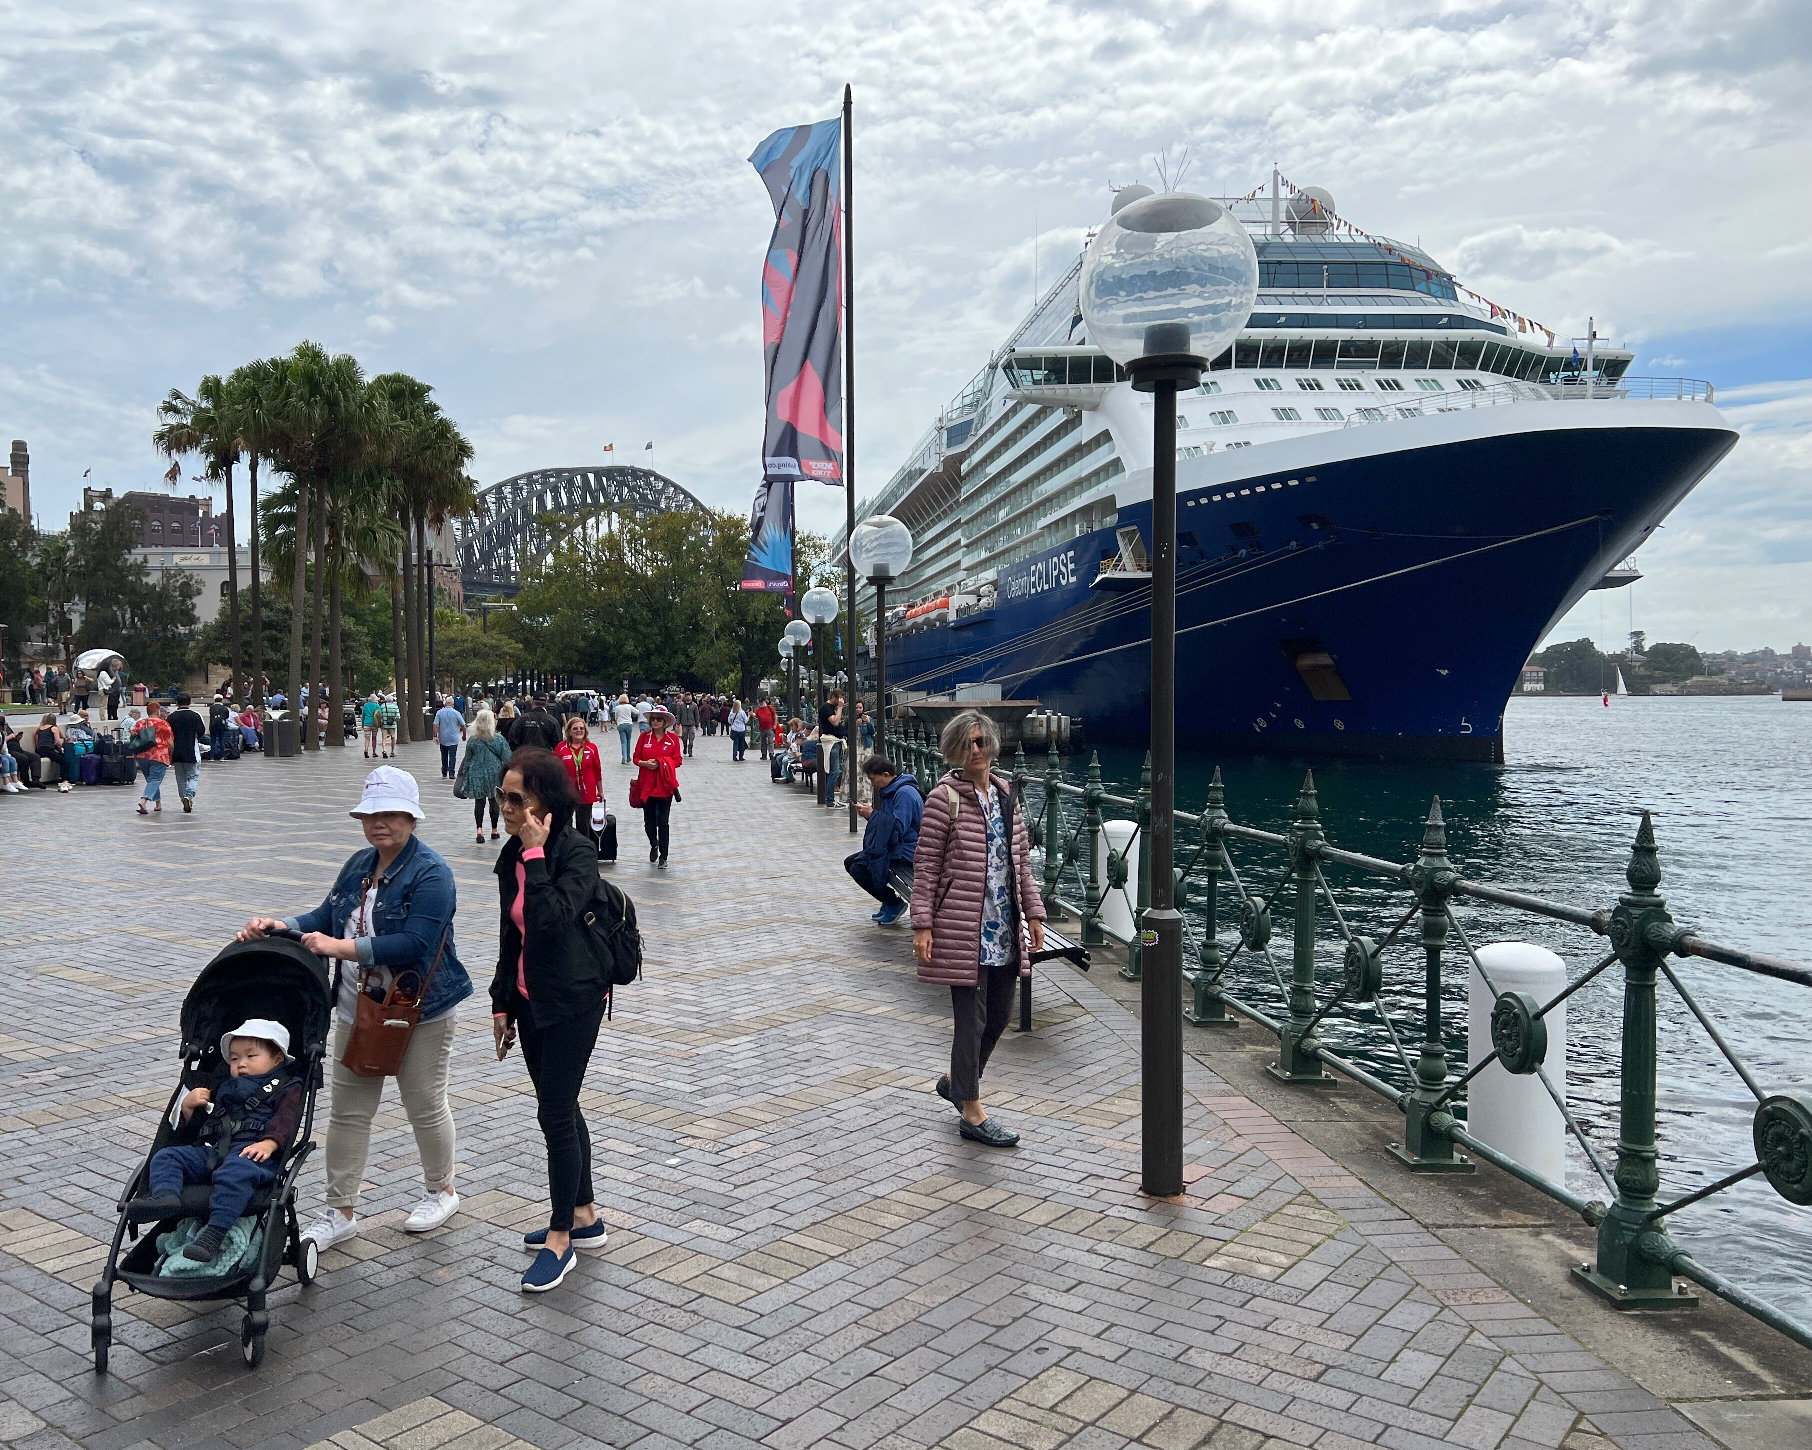
\includegraphics[width=0.40\textwidth]{celebrity-eclipse-sydney-dock.jpg}}
\caption[Our first glimpse of the Celebrity Eclipse]{Our first glimpse of the Celebrity Eclipse. My first thought,
``This thing is as big as the aircraft carrier in the San Diego
harbor.''}
\label{fig:7606x0}
\end{SCfigure}

\hypertarget{day-16-oct-23-2022}{%
\paragraph{\texorpdfstring{\textbf{Day 16 Oct 23, 2022}}{Day 16 Oct 23, 2022}}\label{day-16-oct-23-2022}}

\textbf{Celebrity Eclipse Stateroom 6156, Tasman Sea, Mac}

We are in our Celebrity Eclipse stateroom 6156. Our room is a veranda
room on deck 6. There are 16 levels on the ship and a huge midship show
elevator runs up and down between them. Imagine a Vegas Casino filled
with chubby senior citizens, many using canes and wheelchairs, then put
the casino on a ship and lose it in the ocean. Voila, you've imagined
our cruise. We spent most of yesterday exploring the ship. There is a
lot to see but you quickly run out of places. Tomorrow I am going on a
``Behind the Scenes'' tour where they take you through the working areas
of the ship. The galleries, the engine room, the bridge, the staff
dormitories, and the laundry. I hate to say it but I suspect seeing how
you do laundry for over a thousand people a day is going to be more
interesting than browsing overpriced midship shops. I suspect that we
are not ``cruising people.''

Cruising people like to sit and eat, and eat, and eat, and then float in
hot tubes. The ship has several pools, inside and out, and all the
bubbling hot tubs were filled with obese women and old male porkers. I
swear they displaced most of the tub water. When not displacing tub
water cruising people prowl the forever open buffets to maintain their
hippo-Esque physiques. And when sated with floating and eating, cruising
people lollygag in lounges making an effort to relax. Actual hippos do
it better. Yes, we are probably not cruising people.

This was driven home by the noon art auction. We sat and watched elderly
people pay thousands of dollars for ``art.'' I kept thinking my
daughter's stuff is more interesting and that's not just the dad in me
speaking. After the auction, we had some gelato, ate lunch, found the
exercise room: it's better than most gyms, and then retired to our
stateroom.

The ocean outside our veranda is forever arresting. You wouldn't expect
a flat water-filled horizon to differ from day to day but it does. This
surprised me when I worked on offshore drilling rigs decades ago and
it's still the same. Our departure from Sydney Harbor actually took me
by surprise. The ship moved so smoothly from its berth that I didn't
even notice we had left the dock until I looked up and saw the Sydney
Harbor Bridge. Mali and I were apart during departure. She was elsewhere
on the ship and her pictures of the Sydney Opera House were better than
mine. I went to the front of the ship, and from the solstice deck,
watched the ship follow the little pilot boat out of the harbor. The
blinking green and red buoys looked like an airport runway at night. The
history is wrong, ships were leaving harbors long before planes were
flying. It's more accurate to say an airport runway looks like a harbor
right-of-way.

We didn't eat until 8:30 pm and then we retired to our room. I slept
well, as usual, and Mali did not, also as usual.


\captionsetup[figure]{labelformat=empty}
\begin{figure}[htbp]
\centering
\href{https://conceptcontrol.smugmug.com/Trips/Overseas/Australia-New-Zealand-2022/i-4m5CvVC/A}{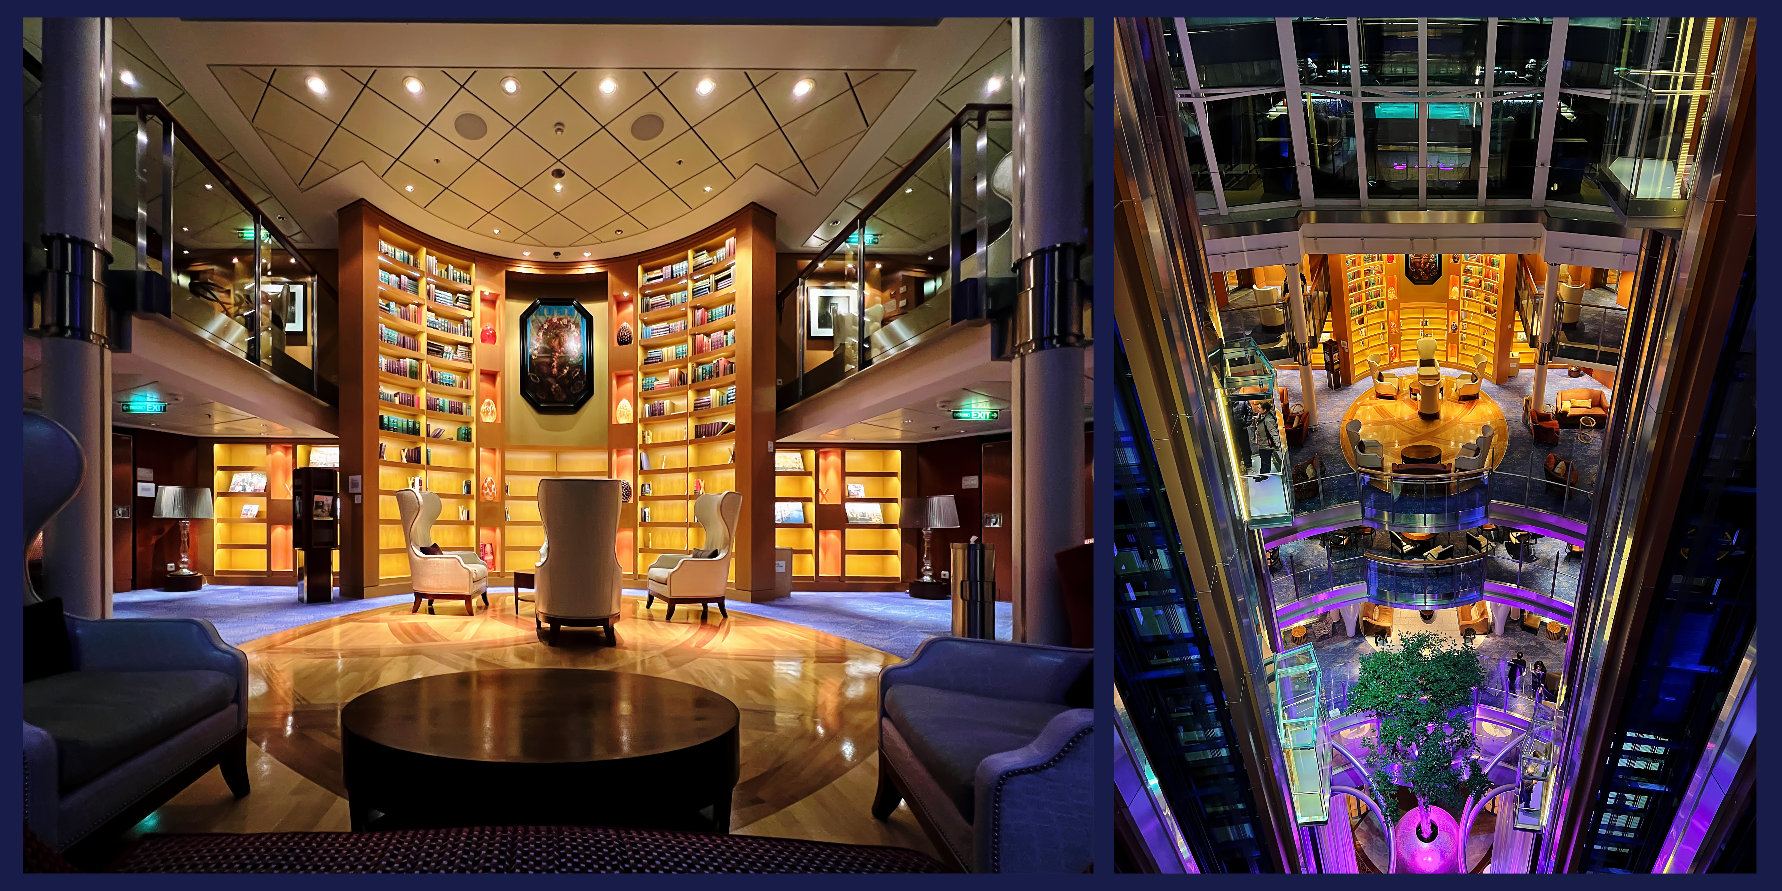
\includegraphics[width=0.75\textwidth]{ship-library-elevator.jpg}}
\caption[Ship library and show elevator]{The ship's interior had its charms. I liked the library and the
main show elevators. At first, I thought the library was an actual
library, but silly me the ``books'' were just for show, and as you see,
most of them were out of reach. The library was a homage to an earlier
epoch when upper-class passengers would dress in suitable attire and
then make a show of how cultured they were. So much of what we consider
``classy'' is an echo from ages that had class, because, let's be
honest, our twerking and ``trumpy'' era has none.}
\label{fig:7606x1}
\end{figure}

\hypertarget{day-17-oct-24-2022}{%
\paragraph{\texorpdfstring{\textbf{Day 17 Oct 24, 2022}}{Day 17 Oct 24, 2022}}\label{day-17-oct-24-2022}}

\textbf{Celebrity Eclipse Stateroom 6156, Tasman Sea, Mac}

We are still some 300 nautical miles from the west coast of New Zealand.
The cruise itinerary is changing en route. I was under the impression we
would be in Milford Sound this morning but it's apparently tomorrow
morning. The weather is expected to be overcast and rainy which may work
to my advantage as it will reduce the number of people on the outer
decks leaving more spots for me to take pictures. Still, this is our
third day at sea and I was expecting only two. Maybe cruises adjust for
weather and port conditions all the time and this is nothing unusual.
The other passengers seem woefully unconcerned. Still, I see why old
ocean liners were so obsessed with speed. It takes forever to get
anywhere on a ship! If the Titanic, (smaller than the ship I am
currently on), hadn't been trying to beat a speed record it wouldn't
have hit that iceberg.

Last night we had dinner in one of the specialty restaurants: \emph{Le
Petit Chef}. I thought it was going to be a standard French Restaurant
but the \emph{Le Petit} bit was literal. A cute series of animated
cartoon characters were projected on the table. It was a surprisingly
high-quality projection. You watched a little French family gather raw
ingredients and build your dinner by throwing projected food on your
plate. When the dinner course animation ended the waiter placed your
actual food in the same spot. It was cute and the food was good.

This morning I wanted to take the ``Behind the Scenes'' tour and I
promptly showed up at 8:30 am at the Shore Excursions desk only to learn
that we had crossed another time zone last night and it was 9:30 am -
not 8:30 am. When flying you zoom through time zones, reset your watch,
and suffer jet lag for a few days. On a ship, you adjust without
noticing it and just miss appointments. I must say I enjoy the relaxed
ship vibe. No white-knuckle sailors are holding onto their spouses and
expecting to sink without warning. Life aboard is super chill. Mali and
I even had boat sex last night. It was the first time we'd had sex on a
moving object; I'm discounting planet Earth. Afterward, I said that most
people don't do \emph{that} on airplanes! Yes, I've heard of the
mile-high club, but non-billionaires don't boink in nice staterooms with
an ocean view.

Today I will probably switch to my wide-angle Nikon lens and shoot some
pictures.

\hypertarget{day-18-oct-25-2022}{%
\paragraph{\texorpdfstring{\textbf{Day 18 Oct 25, 2022}}{Day 18 Oct 25, 2022}}\label{day-18-oct-25-2022}}

\textbf{Celebrity Eclipse Stateroom 6156, New Zealand Coastal Waters, Mac}

We spent the day cruising New Zealand fiord country. Milford Sound,
Doubtful Sound, and Dusky sound. Took lots of pictures.

\captionsetup[figure]{labelformat=empty}
\begin{figure}[htbp]
\centering
\href{https://conceptcontrol.smugmug.com/Trips/Overseas/Australia-New-Zealand-2022/i-8Mw2Rdz/A}{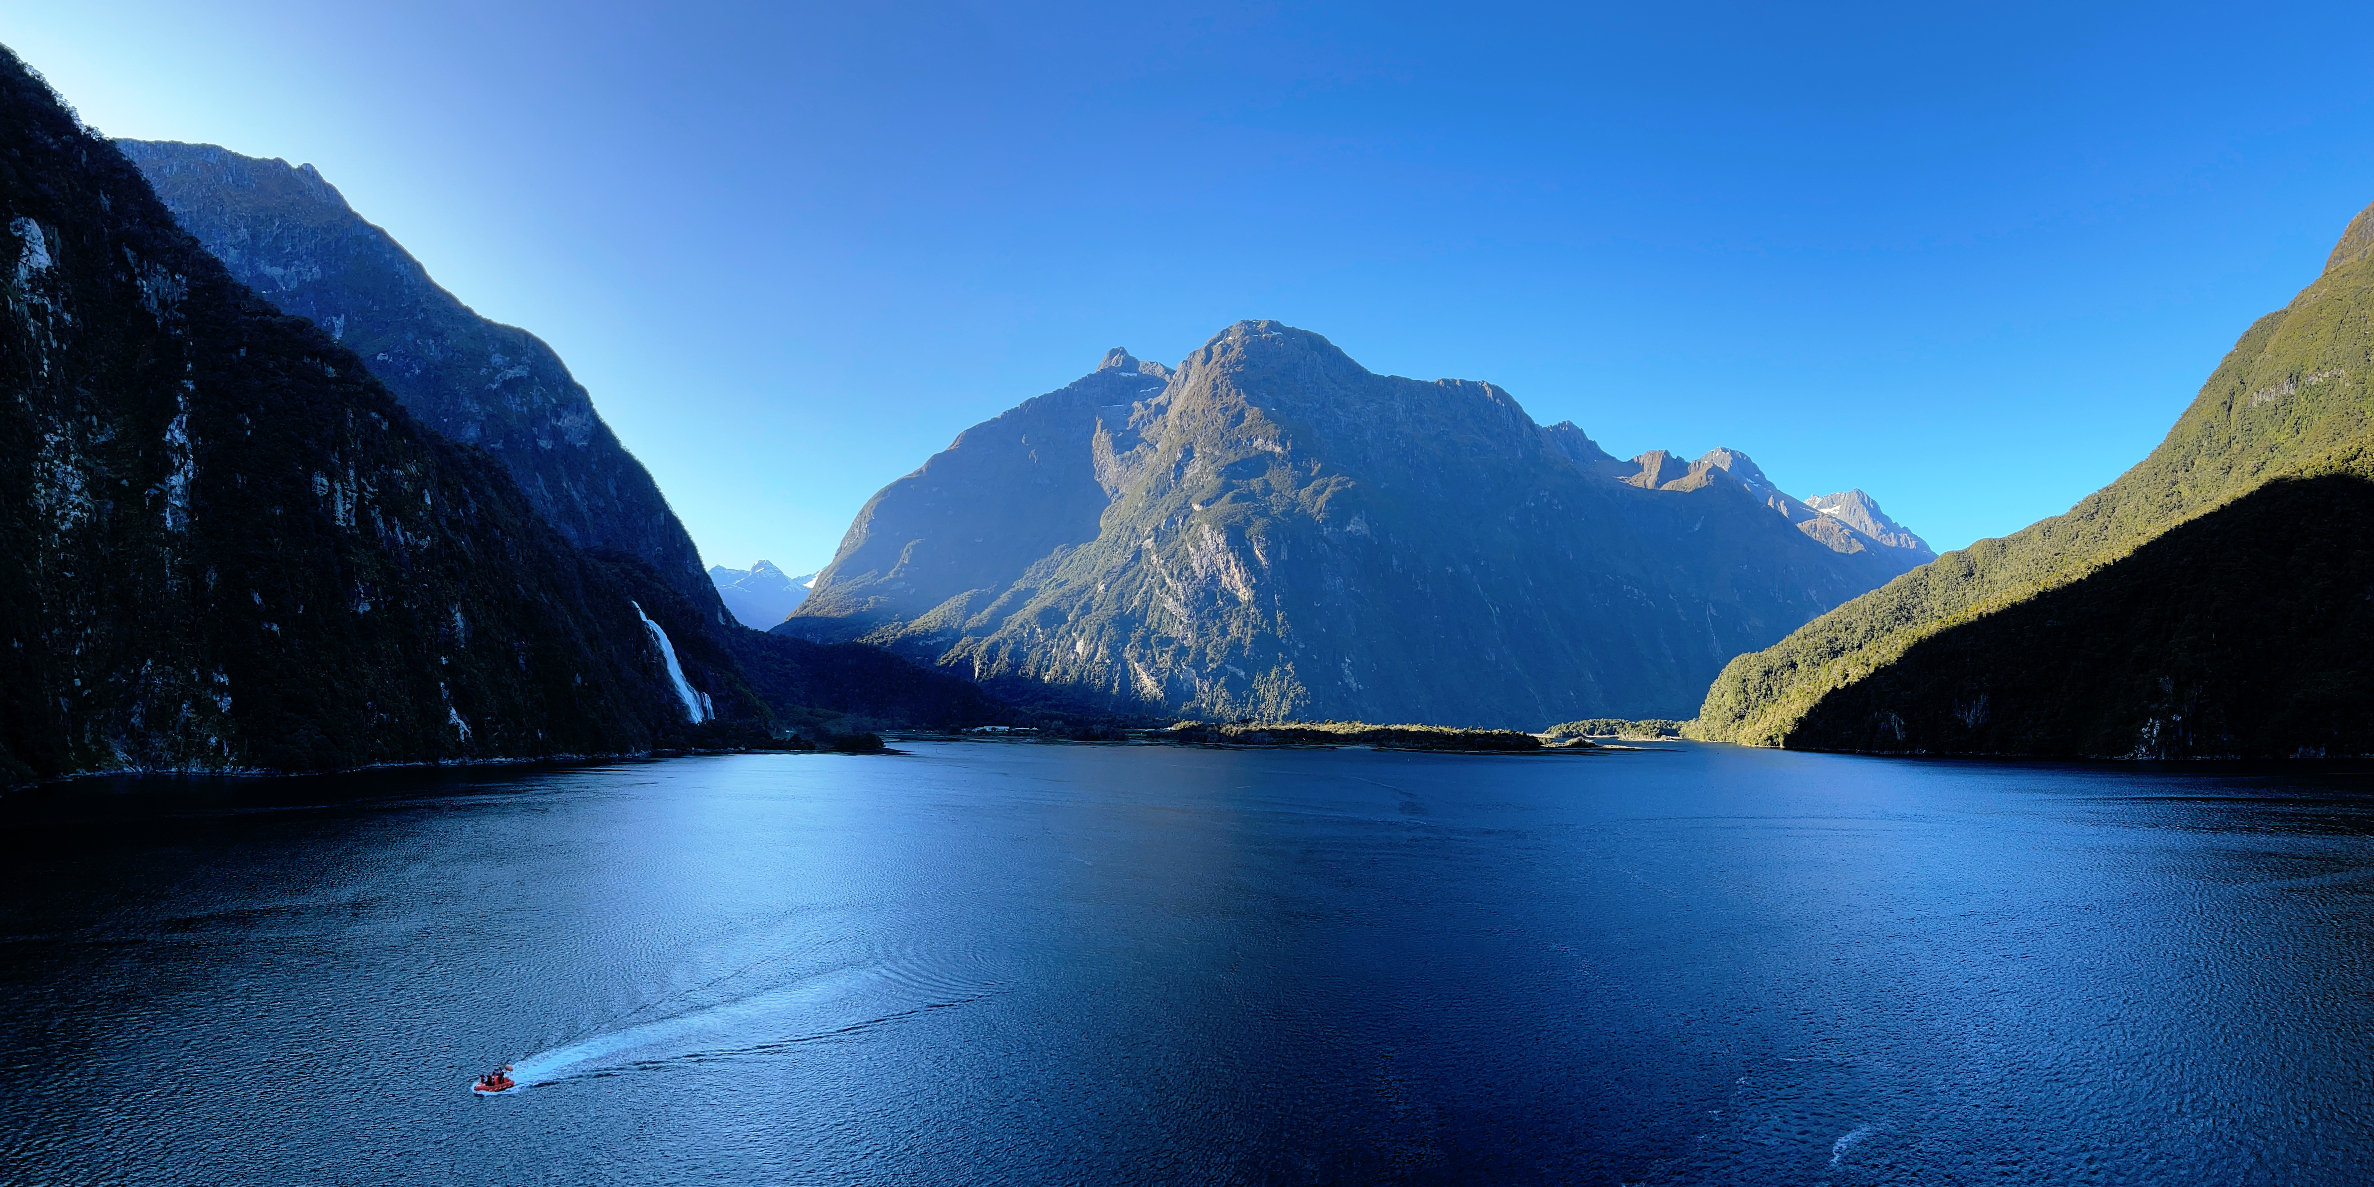
\includegraphics[width=0.80\textwidth]{milford-sound-morning.jpg}}
\caption[Milford Sound in the morning]{Milford Sound in the morning from the upper deck of the cruise
ship. The ship did not dock in the sound. A small boat came alongside,
and a dozen passengers disembarked to go overland to the next stop in
Dunedin. We considered joining them, but the absurdly high cost of one
night in the Fiordlands deterred us.}
\label{fig:7606x2}
\end{figure}

Also, tonight and the previous night, I attended the live shows in the
Eclipse Theatre. The shows are Ok music and stand-up acts.

Too tired to write more. Tomorrow, we go ashore in Dunedin after four
nights on the ship.

\hypertarget{day-1819-oct-2627-2022}{%
\paragraph{\texorpdfstring{\textbf{Day 18,19 Oct 26,27 2022}}{Day 18,19 Oct 26,27 2022}}\label{day-1819-oct-2627-2022}}

\textbf{Celebrity Eclipse Stateroom 6156, New Zealand Coastal Waters, Mac}

The last two days have been shore days. On the 26\textsuperscript{th} we
visited Dunedin. After four nights on the ship, it was nice to get back
on land. Dunedin is a small University City on the South Island of New
Zealand. We didn't sign up for any shore excursions so we hopped on a
local tour at the wharf. We rode in a small
\href{https://awesometours.co.nz/}{Awesome Tours} bus with Mac our
driver. There were only three of us: Mali, myself, and another lady from
Brisbane. It was almost like a private tour. Mac took us downtown, where
we exchanged some US hundreds for New Zealand dollars. Then we were
driven to \href{https://www.larnachcastle.co.nz/}{Larnach Castle}, which
was never actually a castle. It was a country estate built by Larnach in
the 19\textsuperscript{th} century. It was nice but frankly, I wouldn't
recommend the castle. There are lots of nice estates on this planet.

After the castle, we drove up the Dunedin peninsula and had lunch at the
bird sanctuary. There were three varieties of gulls flying and pooping
all over. We didn't see any albatrosses Then we drove up the hill to see
New Zealand seals and Little Blue Penguins. The Little Blue Penguins
were on their nests. They are delightful and were one of the highlights
of this trip. We also saw chicks at various stages of development.


\captionsetup[figure]{labelformat=empty}
\begin{SCfigure}
\centering
\href{https://conceptcontrol.smugmug.com/Trips/Overseas/Australia-New-Zealand-2022/i-mnh9FHw/A}{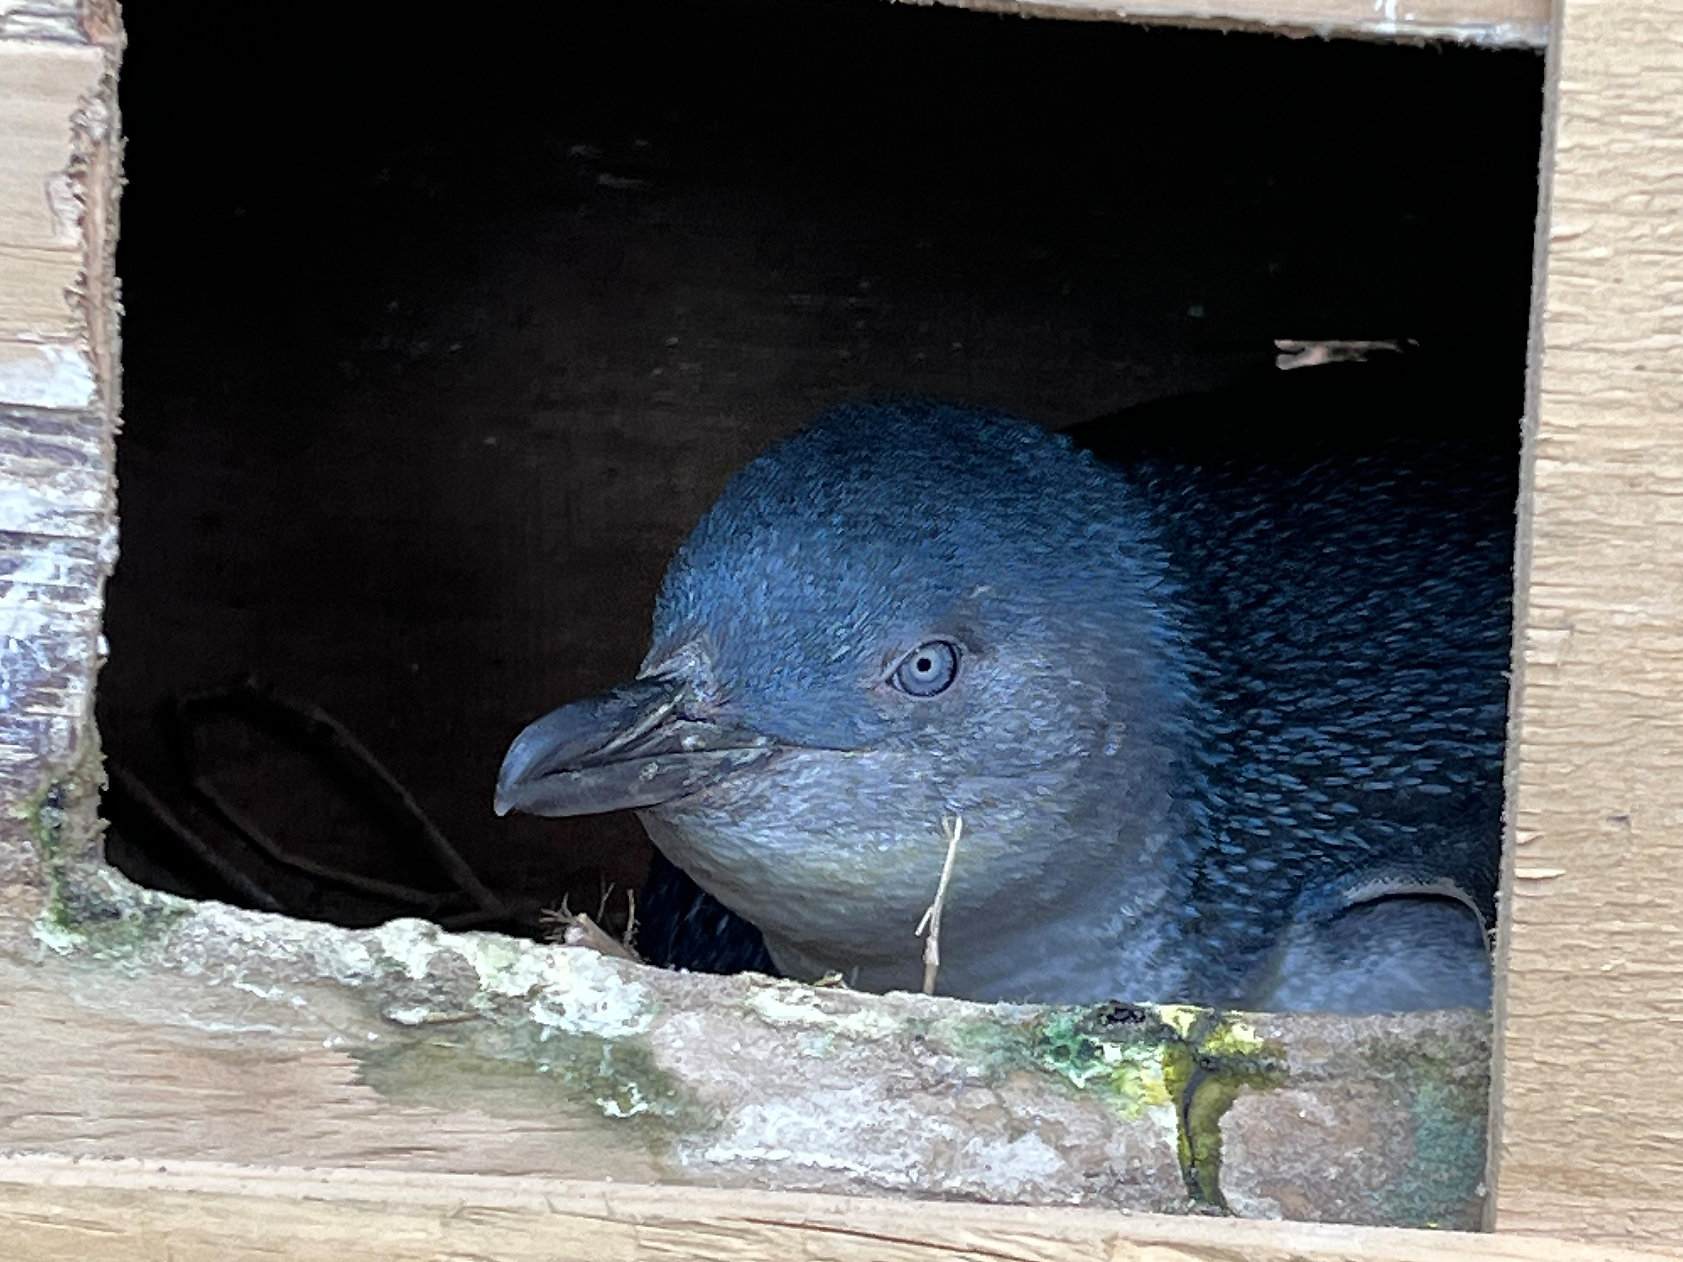
\includegraphics[width=0.40\textwidth]{nesting-blue-penquin.jpg}}
\caption[Nesting blue penguins]{The little blue penguins of New Zealand are avian celebrities.
Everyone loves them, and if you don't, there is something very wrong
with you.}
\label{fig:7606x3}
\end{SCfigure}

After the penguins, we drove to the steepest street in the world. It's
amazing what turns into a tourist attraction. I particularly appreciated
Mac's discussion on how street steepness is measured. In case you're
wondering \emph{Calculus is involved}.

Then it was back to the ship and to bed early.

As the ship left Dunedin, we saw albatrosses gliding around the
sanctuary point. It was the first time I'd seen more than one in the air
at a time.

Today we visited Christchurch New Zealand. The cruise ship docks at both
Dunedin and Christchurch are a fair distance from the city. In Dunedin
Mac drove us to and from the wharf. At Christchurch, we rode the
Celebrity shuttles in and out of town.

Christchurch was hit by a big earthquake in 2011. It was only a 6.1
quake but it was very shallow and very close (less than 7 km) from the
city so it did a lot of damage. The city had to rebuild large chunks of
its downtown. The new buildings are nice and designed to withstand big
earthquakes. There's nothing like a shit-kicking to smarten people up.
We spent the afternoon riding the city trolleys --- some cars are over a
hundred years old --- and walking in the city core. We popped into the
Canterbury Museum, The Botanic Gardens, the Art Museum, and various city
parks.

Highlights --- the tunnel into the city, the restored shopping
districts, and the old restored trolleys.

Postscript:

\begin{enumerate}
\def\labelenumi{\arabic{enumi}.}
\item
  The ship's crew all wear masks and are either south Asian, Latinos, or
  Black. They are also fairly short and impeccably dressed in their
  service uniforms. The cruise customers are almost all white with some
  Asians, many are elderly, and many are overweight. There are two
  visible classes on board.
\item
  Ship Internet is slow or nonexistent.
  \href{https://www.starlink.com/}{Starlink} will significantly improve
  at-sea connections.
\end{enumerate}

\hypertarget{day-20-oct-28-2022}{%
\paragraph{\texorpdfstring{\textbf{Day 20 Oct 28, 2022}}{Day 20 Oct 28, 2022}}\label{day-20-oct-28-2022}}

\textbf{Celebrity Eclipse Stateroom 6156, New Zealand Coastal Waters, Mac}

Today we were in Wellington. Highlights --- the parliament Beehive and
the Wellington Cable car. Mali is not feeling well; she is wearing a
mask in bed and watching soccer while fretting about maybe picking up
COVID. Tomorrow we are in Napier.

\hypertarget{day-21-oct-29-2022}{%
\paragraph{\texorpdfstring{\textbf{Day 21 Oct 29, 2022}}{Day 21 Oct 29, 2022}}\label{day-21-oct-29-2022}}

\textbf{Celebrity Eclipse stateroom 6156, New Zealand Eastern Coastal Waters, iPhone}

We were in Napier today. Mali was sick and stayed onboard. I went ashore
by myself. I rented a bicycle across the street from the shuttle bus ``I
Stop.'' I rode it about 7 km up the coast to the wetlands and then
suffered a flat tire. I walked the bike back to the rental place hiking
through Napier. Shakespeare street saved me a kilometer or so on the
hike back.

After returning the bike I had a flat white and a vegan ``Sammy'' in an
organic store Mali would have liked. Then I walked around town and down
the beach before slurping down some smoothies in a little cafe. Napier
is smaller than the other ports we've visited and the cruise people
stood out downtown. In the other locations, they blended in. Tomorrow is
Tauranga.

\hypertarget{day-222324-nov-2-2022}{%
\paragraph{\texorpdfstring{\textbf{Day 22,23,24 Nov 2, 2022}}{Day 22,23,24 Nov 2, 2022}}\label{day-222324-nov-2-2022}}

\textbf{Celebrity Eclipse Stateroom 6156, Tasman Sea, Mac}

I've been slacking off on my diary entries. This is a catch-up.

On Oct 30 we were in Tauranga which is New Zealand's largest port. The
weather was awful it was pouring rain when we walked down the gangplank
and we were soaked by the time we stepped on our ``Hop On Hop Off'' bus.
Mali wasn't feeling well and shouldn't have come but she wanted to see
the city. It blows to be sick on trips. We rode the bus to a shopping
mall. The bus driver told us the mall was the most popular stop on their
route. People like to check out the shops and see how prices differ from
back home. I get it but malls are malls.

We dried out in the mall and I had another flat white. We then rode the
rest of the bus loop and got back on the ship by noon. We both ended up
napping in our stateroom.

On Oct 31 we were in Auckland or as T-shirt once said ``Sydney for
Beginners.'' We walked around the city, went up the tower, and ended up
in an Art Museum. A few young women were ``singing'' in one of the
galleries. Auckland differs from the other New Zealand ports in that the
dock is right downtown. You could walk off the boat into the middle of
the city. Just like Sydney and San Diego.

On Nov 1 we headed back to Sydney. Last night was the roughest night at
sea. I also took an internal ship tour which turned out to be one of the
best tours of the ship. The bridge was as spacious and luxurious as Star
Trek sets.


\captionsetup[figure]{labelformat=empty}
\begin{figure}[htbp]
\centering
\href{https://conceptcontrol.smugmug.com/Trips/Overseas/Australia-New-Zealand-2022/i-vX9x9tw/A}{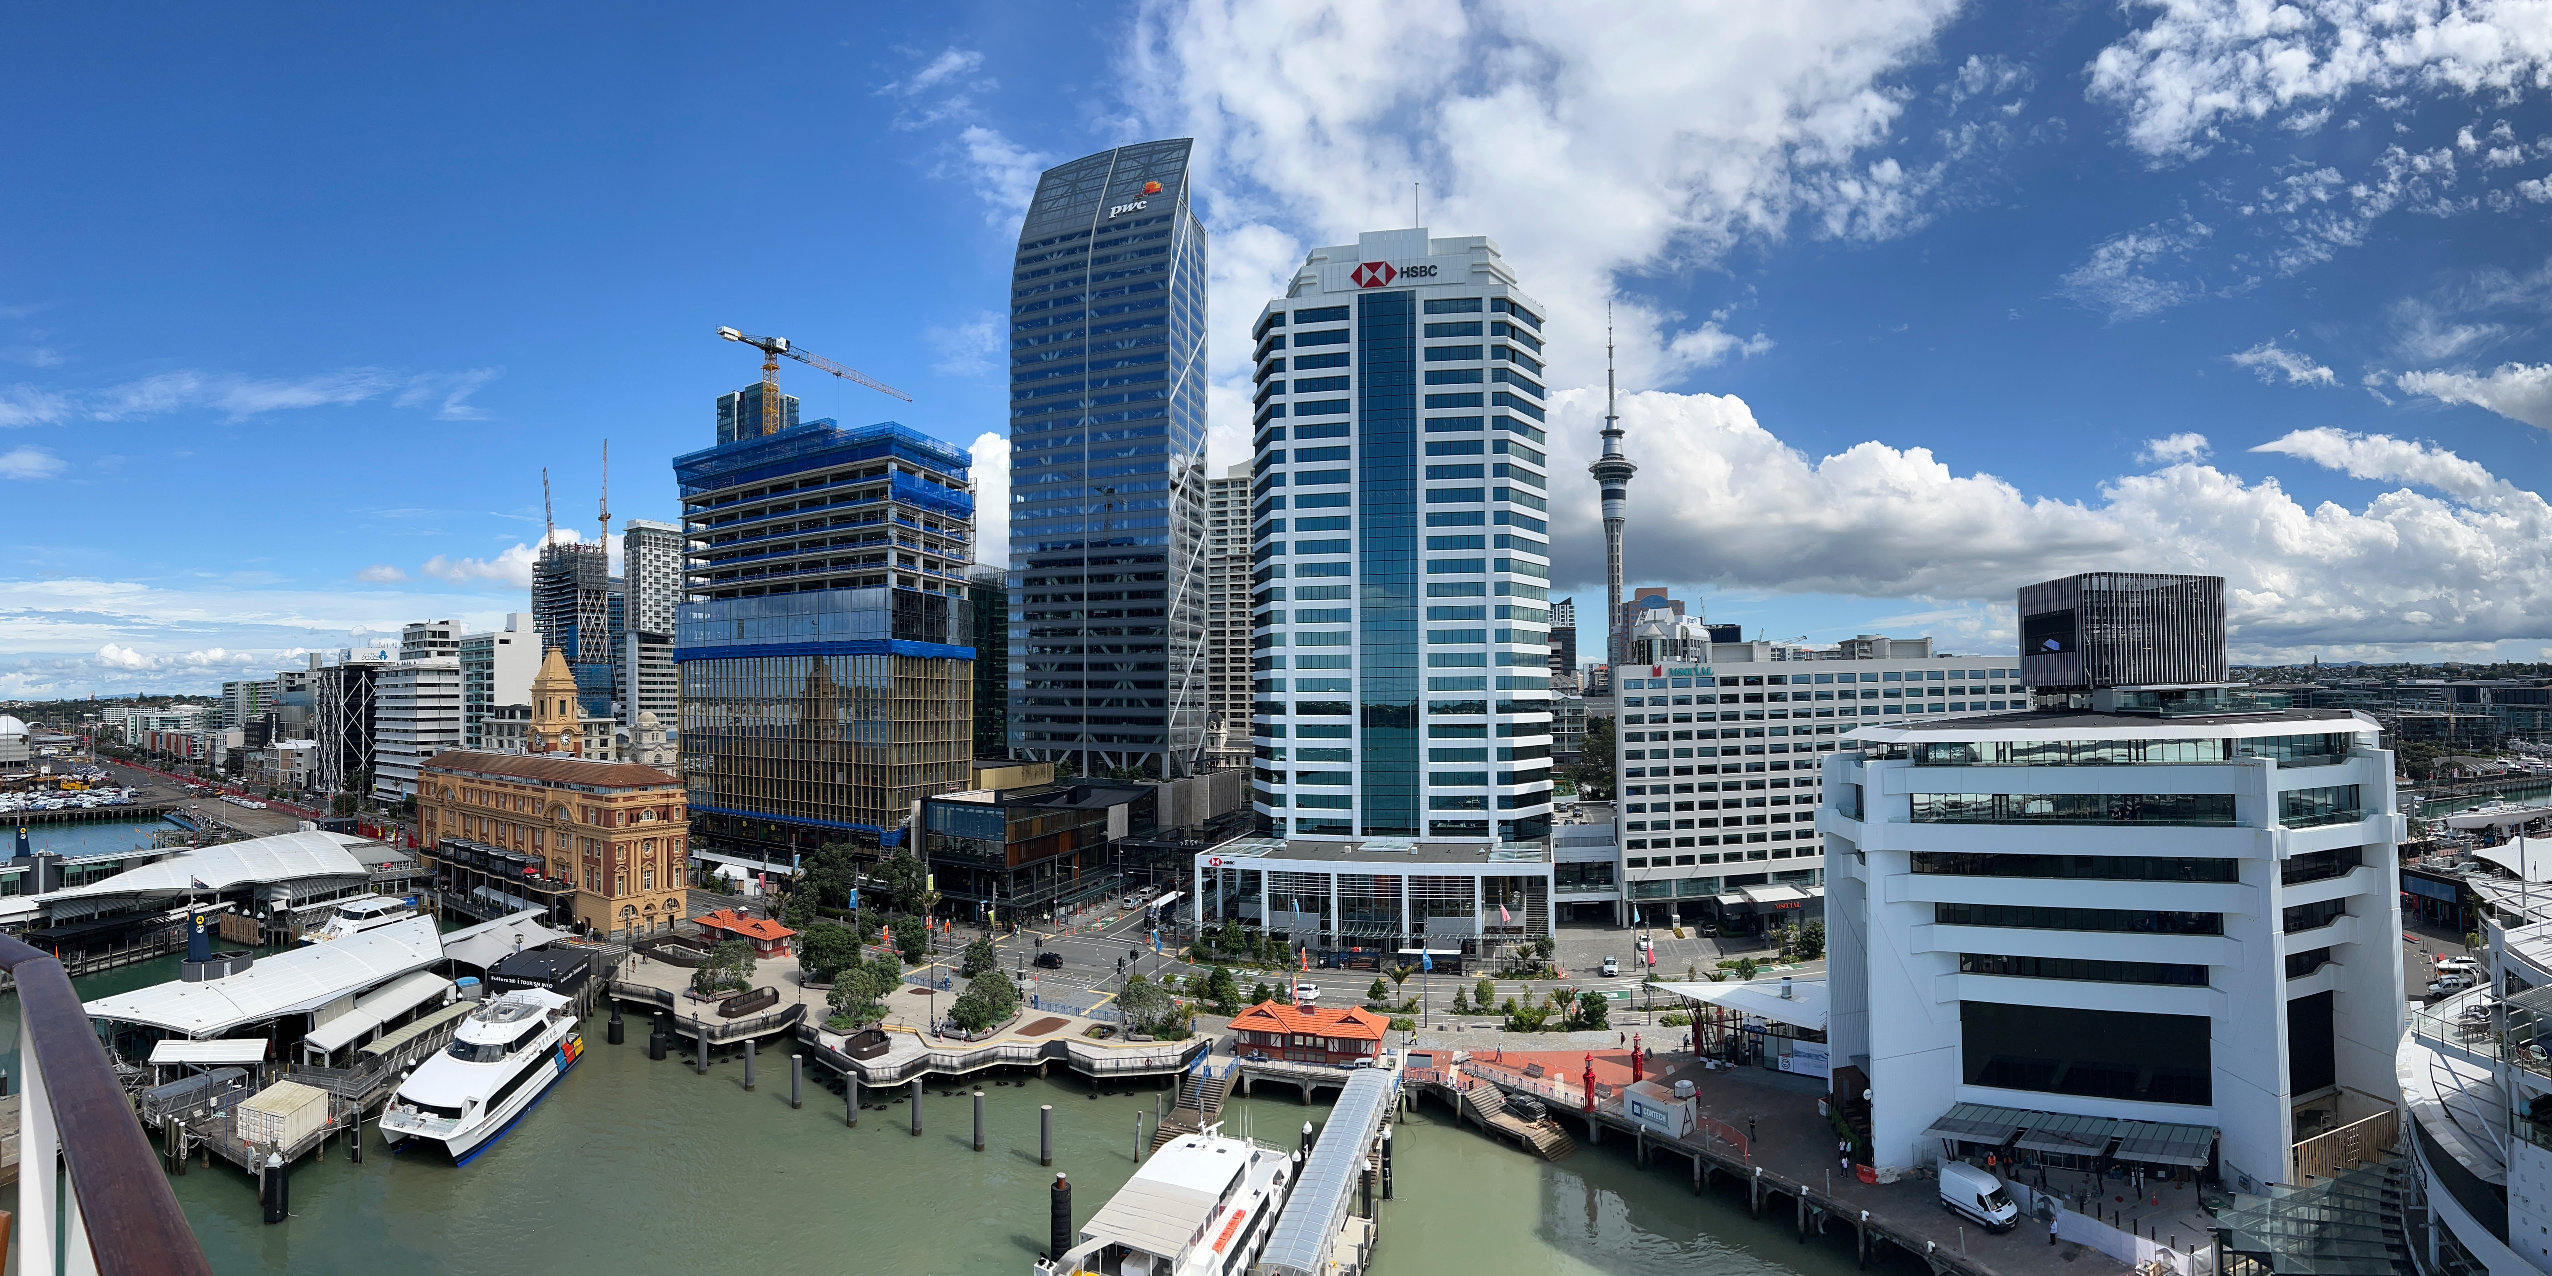
\includegraphics[width=0.80\textwidth]{auckland-downtown-dock.jpg}}
\caption{Auckland from the upper deck of the cruise ship.}
\label{fig:7606x4}
\end{figure}

Postscript:

\begin{enumerate}
\def\labelenumi{\arabic{enumi}.}
\item
  The ship reported a few cases of COVID. The people have been isolated
  and we've been advised to wear masks in public. How this will play out
  when we dock in Sydney remains to be seen. I hope we don't get
  quarantined.
\end{enumerate}


%\end{document}
